\chapter{Modelling word-final /s/ with linear discriminative learning}\label{chapter05}

The aim of the linear discriminative learning implementation presented in this chapter is to further investigate \textsc{H prod\textsubscript{3}}, the ``Emergence Hypothesis".\footnote{An earlier version of this chapter has been published as part of \cite{Schmitz2021b}.} For the production study of Chapter \ref{chapter04}, this hypothesis delivered a rather weak prediction: There are durational differences between different types of word-final /s/. Using an LDL implementation, the nature of these differences is further examined. That is, it is investigated whether measures derived from such an implementation are capable of explaining durational differences between different types of word-final /s/. If so, such measures will potentially provide insight into the underlying effects which lead to such durational differences.

\section{Methodology}\label{section05_1}

The methodology of the present investigation consists of two main stages. First, the implementation of the LDL network itself, including the selection of data to train the network (Sections \ref{section05_1_1} and \ref{section05_1_2}) and the implementation of required matrices (Sections \ref{section05_1_3} to \ref{section05_1_5}). Second, the extraction of several measures derived from the LDL implementation (Section \ref{section05_1_6}), which are then used in the statistical analysis (Section \ref{section05_2}).

\subsection{The semantics of pseudowords}\label{section05_1_1}

The present study follows the implementational basics outlined in Section \ref{section03_3}. However, as /s/ durations in pseudowords (and not in real words) are to be modelled, there are a number of complications. The most important complication arises from the widely shared belief that pseudowords do not have meaning (see Section \ref{section03_1_1} for a more detailed discussion). So how can one map form and meaning with forms that have no, or at least no a priori specified, meaning? In a recent study (\cite{Chuang2021}) it was shown that the assumption that pseudowords are bare of meaning is most probably wrong. Due to their formal similarity with existing words, pseudowords resonate with the lexicon. As a result, they may in fact carry meaning. \citet{Chuang2021} demonstrated that quantitative measures gauging the semantic neighbourhoods of pseudowords predict reaction times of lexical decision and acoustic durations. The present study is inspired by these results and implements a similar architecture. To model resonance of pseudowords with the lexicon, both real words and pseudowords must be included in the network. The following sections will detail the combined LDL implementation of real words and pseudowords.

\subsection{Sets of pseudowords and real words}\label{section05_1_2}

The pseudowords and their phonetic realisations that this study is based on are taken from the study of word-final /s/ production presented in Chapter \ref{chapter04}. As linear discriminative learning (e.g. \cite{Baayen2019}) in its current implementation does not offer the option to integrate clitics, the pseudoword set for the present study was limited to two types of /s/: non-morphemic and plural /s/. Recall that some pseudowords showed a number of different realisations by the participants in the production experiment, e.g. \textit{prups} was sometimes produced as /pɹʌps/ and sometimes as /pɹups/. Thus, not 48 (i.e. the number of pseudowords in their orthographic representation) but 78 different phonological forms were included in the pseudoword data set. Table \ref{tab:5.1} gives an overview of all pseudowords and their phonological forms.

\begin{table}\fontsize{9}{10}
\caption{Overview of all pseudowords and their phonological forms used in the LDL implementation. Transcriptions are given in the DISC keyboard phonetic alphabet (\cite{Burnage1988})}
\label{tab:5.1}
\centering
\begin{tabular}{llllll} 
\lsptoprule
\multicolumn{2}{l}{Pseudoword}                                                          & Phonological form                                                                                     & \multicolumn{2}{l}{Pseudoword}                                                        & Phonological form                                                                                     \\ 
\midrule%\cline{1-2}\cline{3-3}\cline{4-6}
\multirow{4}{*}{blou-} & fs                                                             & blufs                                                                                                 & \multirow{4}{*}{glai-} & fs                                                           & gl1fs                                                                                                 \\
                       & ks                                                             & bl\{ks;
  bluks; blVks                                                                                &                        & ks                                                           & gl1ks;
  gl\{ks                                                                                       \\
                       & ps                                                             & blups                                                                                                 &                        & ps                                                           & gl1ps;
  gl\{ps                                                                                       \\
                       & ts                                                             & bl6ts;
  bluts                                                                                        &                        & ts                                                           & gl1ts;
  gl\{ts; gl2ts                                                                                \\ 
\midrule%\cline{1-2}\cline{3-3}\cline{4-6}
\multicolumn{2}{l}{\begin{tabular}[c]{@{}l@{}}cloo-fs; -ks; \\ -ps; -ts\end{tabular}}   & \begin{tabular}[c]{@{}l@{}}klufs; kluks; \\ klups; kluts\end{tabular}                                 & \multicolumn{2}{l}{\begin{tabular}[c]{@{}l@{}}plee-fs; -ks; \\ -ps; -ts\end{tabular}} & \begin{tabular}[c]{@{}l@{}}plifs; pliks; \\ plips; plits\end{tabular}                                 \\ 
\midrule%\cline{1-2}\cline{3-3}\cline{4-6}
\multicolumn{2}{l}{gli-fs;
  -ks; -ps; -ts}                                             & \begin{tabular}[c]{@{}l@{}}glIfs; glIks; \\ glIps; glIts \\glifs; gliks; \\ glips; glits\end{tabular} & \multicolumn{2}{l}{pru-fs;
  -ks; -ps; -ts}                                           & \begin{tabular}[c]{@{}l@{}}prVfs; prVks; \\ prVps; prVts; \\prufs; pruks; \\ prups; pruts;\end{tabular}  \\
\lspbottomrule%\cline{1-2}\cline{3-3}\cline{4-6}
\end{tabular}
\end{table}

The second set of words contained real words and their phonetic realisations. Following \citet{Chuang2021}, these words were extracted from the MALD corpus (\cite{Tucker2019Brenner}). While the MALD corpus contains 26,793 real words, only a subset of 8,285 words was used for a number of reasons. First, some 7,577 words in the corpus contain multiple affixes. As it was unclear how to handle such words, these were excluded. Second, only words for which there were semantic vectors could be used, leading to the exclusion of further 6,828 words. Third, only words with transcriptions available in the CELEX corpus (Baayen et al., 1995) were retained, i.e. there was no transcription available for 818 words. Fourth, 3,285 words showed ambiguities regarding their morphology, e.g. walks as a third-person singular verb versus the plural of a noun. As huge numbers of words lead to extensive computation times, it was decided to exclude such cases as well. The final set of real words contained 6,165 simple and 2,120 complex word forms.

\subsection{Cue matrices}\label{section05_1_3}

As introduced in Section \ref{section03_3}, cue matrices are coded in binary form, giving information on which triphones are part of which word. For the current implementation, two such cue matrices were created using the \texttt{WpmWithLdl} package’s (\cite{Baayen2019wpm}) \texttt{make\_cue\_matrix} function. First, $C_{rw}$, the real word cue matrix, was created for the set of real words. Then, a second cue matrix, $C_{pw}$, was created for the set of pseudowords. $C_{pw}$ is a lot smaller than $C_{rw}$ as there were only 78 phonological forms for pseudowords, but more than 8,000 for real words. $C_{rw}$ was of dimension $8,285×7,610$, while $C_{pw}$ was of dimension $78×78$. 

\subsection{Semantic matrices}\label{section05_1_4}

To introduce semantics, i.e. semantic vectors, for the present set of real words, a pre-built semantic matrix $A$ from \citet{Baayen2019} was used. These authors derived semantic vectors based on the TASA corpus (\cite{Ivens1991}). For this, words were parsed into their lexomes, i.e. inflected words were represented by their base and sense-disambiguated labels for their respective inflectional functions. Ambiguous forms, e.g. walks, were disambiguated using part of speech tagging (\cite{Schmid1999}). Derived words were assigned a lexome for their base and a lexome for derivational function. Then, following \citet{Baayen2016} and \citet{Milin2017Feldman}, naive discriminative learning (henceforth NDL; \cite{Baayen2011, Sering2018}) was used to build semantic vectors. The Rescorla-Wagner update rule (\cite{Rescorla1972, Wagner1972, Rescorla1988}) was applied incrementally to the sentences of the TASA corpus. That is, for each sentence the algorithm was given the task to predict the lexomes in that sentence from all lexomes of that sentence. This resulted in a $23,562×23,562$ weight matrix $A$. This matrix lists all lexomes as rows and columns. Thus, for a given lexome at row $i$, the association strengths of this lexome with all other lexomes as given as columns is contained. In this state of the $A$ matrix, lexomes predict themselves. Thus, the diagonal of the $A$ matrix is set to zero (see \cite{Baayen2019} for a discussion on this procedure). Lastly, columns which mostly contained zeros, i.e. no information, and showed small variances ($σ<3.4*10^{-8}$) were removed. The resulting $A$ matrix is of dimension $23,562×5,030$. Following the method outlined in Section \ref{section03_3}, a semantic matrix for real words $S_{rw}$ can be constructed based on $A$. That is, the semantic vector $\overrightarrow{s}$ in $S_{rw}$ for a simplex word is identical to its corresponding lexome, while the semantic vector $\overrightarrow{s}$ in $S_{rw}$ for a complex word is the sum of its corresponding lexomes. That is, the semantic vector of \textit{apple} is $\overrightarrow{apple}$, while the semantic vector of \textit{apples} is the sum of the vectors of the lexomes \textsc{apple} and \textsc{plural}, i.e. $\overrightarrow{apples}=\overrightarrow{apple}+\overrightarrow{plural}$. As a set of real words was used, $S_{rw}$ contained only semantic vectors for this set of real words (instead of, e.g., all word forms of the TASA corpus). The final real word semantic matrix $S_{rw}$ was of dimension $8,285×5,487$.

While this procedure is rather straightforward, the creation of a pseudoword semantic matrix $S_{pw}$ is not. Due to the nature of pseudowords, their lexomes are not contained within any corpus or the $A$ matrix, for that matter. Instead, one can estimate a pseudoword’s semantic content by utilising the semantic and phonological information on real words, i.e. their $C$ and $S$ matrix (\cite{Chuang2021}). That is, the same transformation matrix $F$ that is used for mapping real word cues onto predicted real word meanings (see Section \ref{section03_3}) can be used to map pseudoword cues onto their estimated semantics. That is, one must first solve

\begin{equation}
\label{eq:FCSpw}
    F=C'_{rw}S_{rw}
\end{equation}

to obtain $F$. Then, one can make use of the pseudoword cue matrix $C_{pw}$ and estimate pseudoword semantics, as

\begin{equation}
\label{eq:SCFpw}
    S_{pw}=C_{pw}F
\end{equation}

with $S_{pw}$ denoting the originally estimated semantic matrix for pseudowords. In this semantic matrix, pseudowords of identical segmental makeup show identical semantics, as semantics are calculated only based on triphone occurrence, i.e. the semantics of \textit{pleeps\textsubscript{singular}} is identical to the semantics of \textit{pleeps\textsubscript{plural}}. To differentiate between singular and plural pseudowords, the semantic vector of the \textsc{plural} lexome is added to all plural pseudowords in the $S$ matrix. Similarly, the semantic vectors of \textsc{alien} and \textsc{creature} are added to all pseudoword semantic vectors as participants in the original production experiment were told that pseudowords describe alien creatures. As explained in Section \ref{section04_1}, the pairing of the pictures with pseudowords representing the alien creatures was randomised during the experiment. A particular pseudoword thus only contained the semantics of ``alien creature" as a constant part of its own semantics, while other factors such as appearance, e.g. colour, shape, or number of eyes, differed across participants. One may assume that in the course of the experiment, participants gradually came to realise that the looks of these alien creatures, i.e. colour, shape, etc., are not relevant to their label names. Thus, participants were just aware of the fact that these are all alien creatures, without paying much attention to their individual features. Please see the \ref{Supplementary Material} for a detailed implementation.

\subsection{Comprehension and production}\label{section05_1_5}

Pseudoword comprehension and production were not computed and evaluated in isolation, but in combination with real words, simulating a real person’s lexicon in a pseudoword comprehension and production situation, respectively. For this, a cue matrix $C_{comb}$ was created based on a combined set of words, containing all aforementioned real words and pseudowords. In total, 8,440 word forms were part of this set of words. A combined semantic matrix $S_{comb}$ was created by attaching $S_{pw}$ to $S_{rw}$, and reordering its rows to reflect the same order of words as found in $C_{comb}$ using the \texttt{LDLConvFunction} package (\cite{Schmitz2021ldlconv}).

Then, using the \texttt{WpmWithLdl} package (\cite{Baayen2019wpm}), a comprehension model was trained and checked for accuracy. That is, taking form vectors as input for the prediction of semantic vectors of output, $\hat{S}_{comb}=C_{comb}F$ is solved. Comprehension is successfully modelled for a word $i$ if its predicted semantic vector $\hat{s_i}$ is most highly correlated with its targeted semantic vector $s_i$. This is true for 74.41 \% of cases (i.e. 6,165 word forms) in the comprehension model. In total, 25.59 \% of cases (i.e. 2,120 word forms) were incorrectly predicted, with 1,912 simple and 208 complex word forms. None of the incorrectly predicted word forms was a pseudoword.

Similarly, a production model was trained and checked for accuracy using functions of the aforementioned R package. Thus, semantic vectors were provided as input to predict form vectors as output, i.e. to solve $\hat{T}_{comb}=S_{comb}G$. Production was successfully modelled for a word $i$ if its predicted triphones are those triphones present in its targeted cue vector in the correct sequence (possible sequences of triphones will be referred to below as ``paths"). This was true for 97.3 \% of cases (i.e. 8,061 word forms) in the production model. In total, 2.7 \% of cases (i.e. 224 word forms) were incorrectly predicted, with 98 simple and 126 complex word forms. None of the incorrectly predicted word forms was a pseudoword.

\subsection{Measures}\label{section05_1_6}

In order to explore the potential of different measures emerging from the network to predict phonetic duration, a whole range of measures, based on the measures introduced by the \texttt{WpmWithLdl} package (\cite{Baayen2019wpm}) and by \citet{Chuang2021}, were extracted. The measures introduced by \citet{Chuang2021} were extracted using the \texttt{LDLConvFunction} package (\cite{Schmitz2021ldlconv}). Please see the \ref{Supplementary Material} for exploratory analyses of individual measures.

In the following, the semantic measures are described first. Then, the phonetic measures are introduced.

\textsc{l1norm} and \textsc{l2norm}. The \textsc{l1norm} is the sum of the absolute values of vector elements of a given word’s predicted semantic vector $\hat{s}$, i.e. its city-block distance. The \textsc{l2norm} is the square root of the sum of the squared values of a given word’s predicted vector $\hat{s}$, i.e. its Euclidean distance. For both variables, higher values imply more strong links to many other lexomes. Thus, both measures may be interpreted as semantic activation diversity.

\textsc{density}. For \textsc{density}, the correlation values of a word’s predicted semantic vector s ̂ and its eight nearest neighbours’ semantic vectors $s_{n1}...s_{n8}$ are taken into consideration. The mean of these eight correlation values describes \textsc{density}, with higher values indicating a denser semantic neighbourhood.

\textsc{ALC}. The Average Lexical Correlation is the mean value of all correlation values of a pseudoword’s estimated semantic vector as contained in $S_{pw}$ with each of the real word semantic vectors as contained in $S_{rw}$. Higher \textsc{ALC} values indicate that a pseudoword’s semantics are part of a denser semantic neighbourhood. Thus, \textsc{ALC} may be interpreted as a measure of semantic activation diversity for pseudowords.

\textsc{EDNN}. This variable describes the Euclidean Distance of a pseudoword’s estimated semantic vector $s$ and its Nearest semantic real word or pseudoword Neighbour. Thus, higher values indicate a larger distance to the nearest semantic neighbour. \textsc{EDNN} may be regarded as a measure of semantic neighbourhood density.

\textsc{NNC}. The Nearest Neighbour Correlation is computed by taking a pseudoword’s estimated semantic vector as given in $S_{pw}$ and checking it for the highest correlation value against all real word semantic vectors as given in $S_{rw}$. This highest correlation value is taken as \textsc{NNC} value. Thus, higher values indicate that a pseudoword is semantically close to a real word. Additionally, one can tell which real word a pseudoword’s semantics are closest to. This measure may be interpreted as a measure of similarity between pseudo- and real words, indicating the co-activation of a real word when confronted with a pseudoword. 

\textsc{support}. This measure describes the amount of support the word-final triphone (i.e. fs\#, ks\#, ps\#, ts\#) obtains for each pseudoword. The value of \textsc{support} is extracted from $\hat{T}$. Higher values of this variable indicate a higher semantic support for the word-final triphone which includes the segment of interest, i.e. word-final /s/.

\textsc{path\_counts}. \textsc{path\_counts} describes the number of paths, i.e. possible sequences of triphones, detected for the production of a word by the production model. \textsc{path\_counts} may be interpreted as a measure of phonological activation diversity, as higher values indicate the existence of multiple candidates (and thus paths) in production. 

\textsc{path\_sum}. \textsc{path\_sum} describes the summed support of paths for a predicted form. \textsc{path\_sum} may be interpreted as a measure of phonological certainty, with higher values indicating a higher certainty in the candidate form.

\textsc{path\_entropies}. \textsc{path\_entropies} contains the Shannon entropy values that are calculated over the path supports of the predicted form in $\hat{T}$. Thus, \textsc{path\_entropies} may be interpreted as a measure of phonological uncertainty, with higher values indicating a higher level of disorder, i.e. uncertainty.

\textsc{ALDC}. The Average Levenshtein Distance of all Candidate productions is the mean of all Levenshtein distances of a word and its candidate forms. That is, for a word with only one candidate form, the Levenshtein distance between that word and its candidate form is its \textsc{ALDC}. For words with multiple candidates, the mean of the individual Levenshtein distances between candidates and targeted form constitutes the \textsc{ALDC}. Thus, higher values indicate that a word’s candidate forms are very different from the intended pronunciation. \textsc{ALDC} may be interpreted as a measure of phonological neighbourhood density as it takes into account real word neighbourhoods for pseudowords, i.e. large values indicate sparse real word neighbourhoods.

\section{Analysis}\label{section05_2}

Recall that the data set of the production study (Chapter \ref{chapter04}) contains non-morphe-mic, plural, and clitic word-final /s/ as final segment of a pseudoword. As mentioned in Section \ref{section05_1_2}, the present LDL implementation does not include information on clitics. Thus, only durational data on non-morphemic and plural /s/ for the present study are considered. A subset of 666 data points remains, with 303 observations with non-morphemic /s/ and 363 observations with plural /s/. Due to some variable pronunciations requiring triphones not included in the present LDL implementation, 13 data points had to be excluded, resulting in a final data set with non-morphemic and plural /s/ durations of 653 data points, i.e. 300 entries on non-morphemic /s/ and 353 entries on plural /s/. The data set and the following analysis can be found in the \ref{Supplementary Material}.

\subsection{Covariates}\label{section05_2_1}

Besides the aforementioned variables extracted and computed from the LDL implementation itself (see Section \ref{section05_1_6}), the following covariates, adopted from the production experiment (see Section \ref{section04_2_1}) were included in the analysis. The main reason for this is to allow for the comparison of the performance of these predictors with the performance of LDL predictors. LDL measures often correlate with traditional measures (such as lexical frequencies, transitional probabilities, or neighbourhood densities), but the traditional measures have no clear correlating mechanisms in learning or processing.

There are, however, also covariates that do not tap into lexical properties, but that control for other influences, such as speech rate, the speaker, gender, the order of stimuli in an experiment, etc. These will be referred to as ‘non-lexical covariates’ and they will also be included in regression models. 

For reasons of convenience, I will repeat the covariates adopted from the production experiment and their definitions in a shortened version in the following. See Section \ref{section04_2_1} for a detailed account.

\textsc{typeOfS}. This is the explanatory variable of the production study. As the present data set contains only two types of word-final /s/, this binary variable codes whether the pertinent pseudoword is a singular or plural form. It takes the value nm for pseudowords with a non-morphemic word-final /s/ and pl for pseudowords with a plural word-final /s/.

\textsc{speakingRate}. The speaking rate was computed as the number of syllables in an utterance divided by the duration of the utterance.

\textsc{baseDurLog}. Indicating a more local speaking rate, base duration was measured. The base duration in this case is equal to the summed duration of all word-internal segments preceding the /s/ under investigation. The base duration was log-transformed and centred. This variable is called \textsc{baseDurLog}.

\textsc{pauseBin}. In order to account for final-lengthening effects, all stretches of silence between the offset of the word-final /s/ and the onset of the following word were measured. Silence of 50 ms and above was considered as pause. The closure durations of following plosives were taken into account. Following the results of the production study, pause information was included as binary variable with the values \texttt{pause} versus \texttt{no\_pause}.

\textsc{transcription}. As some pseudowords were produced with multiple pronunciations, their transcription was incorporated as a categorical variable.

\textsc{biphoneProbSumBin}. A binary covariate based on the summed biphone probability was used as a measure of contextual predictability.

\textsc{list} \& \textsc{slideNumber}. To account for possible durational differences due to priming and similar effects, the list number (1 to 12) and the point of occurrence during the experiment of the individual item were also included.

\textsc{preC}. It has been shown that the consonant preceding word-final /s/ may influence the duration of word-final /s/. The consonant preceding the final /s/ was therefore included as a covariate, \textsc{preC}.

\textsc{biphonePron}. The probability of the final biphones /fs/, /ks/, /ps/ and /ts/ in monomorphemic words is included as covariate to account for potential effects of phonotactics.

\textsc{folType}. To account for potential effects of the following word on the duration of /s/, the following word was included in regard to its onset segment adjacent to the word-final /s/. This information was included in form of its segmental class in \textsc{folType}.

\textsc{speaker} \/ \textsc{age}. \textsc{speaker} ID was included to account for inter-speaker differences in production. \textsc{age} was included as well as it may show an influence on phonetic realisations.

\textsc{gender} \/ \textsc{location} / \textsc{monoMultilingual}. Participants’ \textsc{gender} and whether they had grown up in London or elsewhere in South Britain (\textsc{location}) were included as well as they may influence phonetic realisations. Additionally, participants who were early bilinguals (i.e. the L2 was/the L2s were acquired as a pre-school child) were categorised as multilingual, while all other participants were categorised as monolingual in \textsc{monoMultilingual}.

Finally, one additional covariate was introduced, following the discussion of the production experiment.

\textsc{real}. Some of the pseudowords used here and in the production experiment have an orthographically different, but phonologically identical real word counterpart (see Section \ref{section04_4}). The variable REAL was introduced to control for this potential confound. This variable is \texttt{TRUE} for pseudowords with such a real word counterpart, and \texttt{FALSE} for those without. The following pseudowords were considered to show such counterparts: \textit{pleet(s)} corresponds to \textit{pleat(s)}, \textit{glits} corresponds to \textit{glitz}, and \textit{gliks} corresponds to the plural of the surname \textit{Glick} (as in \textit{the Glicks live next door}), whereas \textit{glif(s)} corresponds to \textit{glyph(s)}, which has a very low frequency and thus may constitute a pseudoword for most of the participants.\footnote{Note that in \citet{Schmitz2021b} a slightly different set of pseudowords was considered to have real word counterparts, i.e. \textit{pleets}, \textit{glits}, \textit{glaiks} (instead of \textit{glik}), and \textit{glifs}. The analysis presented here uses the set of pseudowords given in the main text. Results reported here and in \citet{Schmitz2021b} do not differ significantly; all effects show into the same directions.}  

All of the following analyses make use of the following non-lexical covariates: \textsc{baseDurLog}, \textsc{speakingRate}, \textsc{slideNumber}, and \textsc{pauseBin} as variables concerning speech rate and continuity, \textsc{preC} and \textsc{folType} accounting for coarticulatory effects, \textsc{list} taking into consideration potential priming effects, \textsc{monoMultilingual}, \textsc{gender}, \textsc{location}, \textsc{age}, and \textsc{speaker} to account for speaker-individual differences, and \textsc{real} to include effects of real word counterparts.

\subsection{Overview of the data}\label{section05_2_2}

An overview of all variables is given in Table \ref{tab:5.2} and Table \ref{tab:5.3}.

\begin{table}\fontsize{10}{11}
\caption{Summary of the dependent variable and the numerical variables used in the modelling processes}
\label{tab:5.2}
\centering
\begin{tabular}{lrrrr} 
\lsptoprule
Dependent variable  & Mean   & St. Dev. & Min     & Max     \\ 
\midrule
\textsc{sDurLog}             & -2.116 & 0.388    & -3.361  & -1.221  \\ 
\midrule
Numerical variables & Mean   & St. Dev. & Min     & Max     \\ 
\midrule
\textsc{speakingRate}        & 3.566  & 0.927    & 1.310   & 7.100   \\
\textsc{baseDurLog}          & -1.203 & 0.232    & -1.987  & -0.375  \\
\textsc{biphoneProb}         & 0.001  & 0.002    & 0.000   & 0.004   \\
\textsc{age}                 & 28.470 & 9.323    & 19.000  & 58.000  \\
\textsc{Component1}          & 0.000  & 1.975    & -17.748 & 2.509   \\
\textsc{Component2}          & 0.000  & 1.959    & -2.832  & 11.989  \\
\textsc{Component3}          & 0.000  & 1.488    & -4.312  & 2.983   \\
\textsc{Component.woA.1}     & 0.000  & 1.973    & -18.860 & 2.178   \\
\textsc{Component.woA.2}     & 0.000  & 1.957    & -10.011 & 2.894   \\
\textsc{Component.woA.3}     & 0.000  & 1.487    & -4.175  & 2.928   \\
\textsc{Component.woA.4}     & 0.000  & 1.269    & -3.608  & 3.076   \\
\lspbottomrule
\end{tabular}
\end{table}


\begin{table}\fontsize{10}{11}
\caption{Summary of categorical predictors and the explanatory variable of interest in the final data set}
\label{tab:5.3}
\centering
\begin{tabular}{ll}
\lsptoprule
Categorical variables & Levels                                                   \\
\midrule
\textsc{typeOfS}               & \texttt{nm}: 300~ ~ ~ \texttt{pl}: 353                                     \\
\textsc{pauseBin}              & \texttt{no}: 412~ ~ ~ \texttt{yes}: 241                                    \\
\textsc{transcription}         & 38                                                       \\
\textsc{biphoneProbSumBin}     & \texttt{high}: 161~ ~ ~ \texttt{low}: 492                                  \\
\textsc{list}                  & 12                                                       \\
\textsc{slideNumber}           & 48                                                       \\
\textsc{preC}                  & \texttt{f}: 156~ ~ ~ \texttt{k}: 169~ ~ ~ \texttt{p}: 164~ ~ ~ \texttt{t}: 164               \\
\textsc{folType}               & \texttt{APP}: 190~ ~ ~ \texttt{F}: 11~ ~ ~ \texttt{N}: 106~ ~ ~ \texttt{P}: 165~ ~ ~ \texttt{V}: 181  \\
\textsc{speaker}               & 40                                                       \\
\textsc{gender}                & 2                                                        \\
\textsc{location}              & \texttt{London}: 392~ ~ ~ \texttt{elsewhere}: 261                          \\
\textsc{monoMultilingual}      & \texttt{monolingual}: 532~ ~ ~ \texttt{multilingual}: 121                  \\
\textsc{real}                  & \texttt{FALSE}: 542~ ~ ~ \texttt{TRUE}: 111                               \\
\lspbottomrule
\end{tabular}
\end{table}

\subsection{Modelling strategy}\label{section05_2_3}

Three kinds of models were devised. First, a baseline model with the traditional predictor variables (plus the non-lexical covariates). Second, a model with LDL predictors that also includes \textsc{typeOfS} as a covariate (plus the non-lexical covariates). Third, a model that contains only the LDL predictors (plus the non-lexical covariates).

The three kinds of models will allow answering the given research question. Recall that the ultimate goal is to understand how systematic durational differences emerge between words of different, but homophonous morphological categories. Traditional lexical variables are predictive but cannot explain how morphology can make its way into durational differences. But these models can show that such differences exist by looking at the effect of the variable \textsc{typeOfS}. This is the baseline model. As an alternative, a model that uses LDL measures is implemented. If these measures are predictive, they offer an explanation of the morphologically-induced phonetic differences: They emerge as a by-product of the association of form and meaning in the mental lexicon, and this association is the outcome of discriminative learning. By having a model that also includes \textsc{typeOfS} as an additional predictor, one can see whether the LDL measures completely capture the morphological effect, or whether there is a residue of morphological information that is predictive of duration but is still not captured by the LDL measures.

\subsection{Model A: Traditional measures}\label{section05_2_4}

This model is meant to resemble those in previous studies on word-final /s/ duration (e.g. \cite{Plag2017}), with a special focus on the model found in the production study (see Section \ref{section04_2_4}). Thus, an LMER model was fitted with similar variables and similar effect structures: \textsc{typeOfS}, \textsc{biphoneProbSumBin}, and \textsc{biphoneProb}, as well as those control variables included in all analyses of this study. None of these covariates showed high correlation coefficients. Hence, no cautionary measures regarding collinearity were required before an initial full model was constructed. Following standard procedures to reduce the potentially harmful effect of skewed distributions in linear regression models (e.g. \cite{Winter2019}), the dependent variable, duration of /s/, was log-transformed. The name of this variable is \textsc{sDurLog}. The model selection process proceeded as explained in Section \ref{section03_2_1}. That is, non-significant variables were excluded in a controlled step-wise fashion. 

Then, variance inflation factors (VIFs) were checked. The covariates \textsc{biphone-Prob} and \textsc{preC} showed high VIF values (i.e. $46.53$ and $46.88$, respectively), indicating potential overfitting of the model (e.g. \cite{Zuur2010, Fox2019}). Consequently, \textsc{preC} was removed from the model as it showed the highest VIF value, following the procedure described by \citet{Zuur2010}. Re-fitting the model without \textsc{preC} and re-checking the new variance inflation factor values revealed only non-problematic values. 

Finally, the resulting model’s residuals were trimmed, following the reasoning given in Section \ref{section03_2_1}. This procedure led to a loss of 4 data points, i.e. 0.61 \% of all data points.

\subsection{Model B: LDL measures and \textsc{typeOfS} specification}\label{section05_2_5}

This model makes use of all LDL measures as well as of the \textsc{typeOfS} variable. Additionally, the non-lexical covariates are included. When fitting a model with such a multitude of variables, collinearity is an issue to consider. Following the procedure given in Section \ref{section03_2_3}, all covariates were checked for correlation using the \texttt{SfL} package (\cite{Schmitz2021sfl}). This correlation check resulted in eight correlation coefficients indicating a high degree of correlation, for which the threshold was assumed to be $|rho|≥0.5$. The pairs of correlated covariates as well as their correlation coefficients are given in Table \ref{tab:5.4}.

\begin{table}\fontsize{10}{11}
\caption{Correlated variables and their correlation coefficients}
\label{tab:5.4}
\centering
\begin{tabular}{llrllr} 
\lsptoprule
Variables       & ~               & \textit{rho} & Variables       & ~       & \textit{rho}  \\ 
\midrule
\textsc{l1norm}          & \textsc{l2norm}          & 0.98         & \textsc{typeOfS}         & \textsc{NNC}     & -0.89         \\
\textsc{path\_counts}    & \textsc{path\_entropies} & 0.95         & \textsc{path\_counts}    & \textsc{support} & -0.65         \\
\textsc{path\_counts}    & \textsc{ALDC}            & 0.89         & \textsc{path\_sum}       & \textsc{support} & 0.73          \\
\textsc{path\_entropies} & \textsc{ALDC}            & 0.90         & \textsc{path\_entropies} & \textsc{support} & -0.63         \\
\lspbottomrule
\end{tabular}
\end{table}

Due to the high number of correlated variables, a principal component analysis was used (PCA; see Section \ref{section03_2_3} for further details) to address collinearity issues. In a PCA, the dimensionality of the data is reduced by transforming the included variables into principal components. These transformations result in linear combinations of the predictors that are orthogonal to each other. Thus, the resulting principal components are not correlated. All variables given in Table \ref{tab:5.4} were included in the computation of the principal component analysis, which yielded nine principal components. 

The next step of the PCA is to determine how many of these principal components are meaningful and thus should be retained for further use. Following the criteria given in Section \ref{section03_2_3}, the following was found. First, any component that displays an Eigenvalue greater than $1$ accounts for a greater amount of variance than had been contributed by one variable. Such a component is therefore potentially meaningful. This is true for components 1, 2, and 3. Second, one should retain enough components so that the cumulative percentage of variance explained is equal to at least 80 \%. This, again, is true for components 1, 2, and 3. Third, only interpretable components are to be retained. This, once again, is true for components 1, 2, and 3. Therefore, components 1 to 3 are retained for further analysis, all of which show an Eigenvalue greater than $1$, account for more than 80 \% of variance, and contain strong representations of variables in their loadings.\footnote{In addition, a cluster analysis was performed. This analysis revealed clusters which align well with the retained components of the principal component analysis. The cluster analysis can be found in the \ref{Supplementary Material}.} But what do these principal components mean? The highest loadings of the principal components, i.e. the correlation of the original variables to the pertinent component, are given in Table \ref{tab:5.5}.

\begin{table}\fontsize{10}{11}
\caption{Loadings of original predictor variables in the three retained principal components of the principal component analysis for model B}
\label{tab:5.5}
\centering
\begin{tabular}{lrrr} 
\lsptoprule
~               & \textsc{Component1} & \textsc{Component2} & \textsc{Component3}  \\ 
\midrule
\textsc{l1norm}          & ~          & 0.397      & 0.348       \\
\textsc{l2norm}          & ~          & 0.405      & 0.363       \\
\textsc{path\_counts}    & 0.813      & ~          & ~           \\
\textsc{path\_entropies} & 0.828      & ~          & ~           \\
\textsc{path\_sum}       & -0.430     & ~          & ~           \\
\textsc{ALDC}            & 0.710      & ~          & ~           \\
\textsc{NNC}             & ~          & 0.698      & ~           \\
\textsc{support}         & -0.650     & ~          & ~           \\
\textsc{typeOfS}           & ~          & 0.421      & 0.517       \\
\lspbottomrule
\end{tabular}
\end{table}

\textsc{Component1}. \textsc{Component1} is most strongly positively correlated with \textsc{path\_counts}, \textsc{path\_entropies}, and \textsc{ALDC}, while it is most strongly negatively correlated with \textsc{path\_sum} and \textsc{support}. For \textsc{path\_counts}, higher values indicate the existence of multiple candidates (and thus paths) in production. It hence functions as an indicator of phonological uncertainty. Values of \textsc{path\_entropies} relate to the level of uncertainty concerning the path supports of the predicted candidate form, with higher values indicating a higher level of uncertainty. For \textsc{ALDC}, higher values mean that a word’s candidate forms are very different from the intended pronunciation, indicating uncertainty in production. \textsc{path\_sum} describes the summed support of paths for a predicted form, with higher values indicating a higher certainty in the candidate form. Higher values for \textsc{support} suggest more certainty in the choice of the word-final triphone. \textsc{Component1} can thus be described as a dimension that represents phonological or articulatory certainty.

\textsc{Component2}. \textsc{Component2} is most strongly correlated with \textsc{l1norm}, \textsc{l2norm}, \textsc{NNC}, and \textsc{typeOfS}. \textsc{l1norm} and \textsc{l2norm} both imply more strong links to many other lexomes with higher values indicating a higher semantic activation diversity. Higher values of \textsc{NNC} suggest a close real word neighbour, which leads to higher levels of co-activation of that real word when confronted with the pseudoword, also leading to higher semantic activation diversity. As for \textsc{typeOfS}, \textsc{Component2} is positively correlated with the presence of non-morphemic /s/ data points. 

\textsc{Component3}. \textsc{Component3} is similar to \textsc{Component2} as it is also strongly correlated with \textsc{l1norm}, \textsc{l2norm}, and \textsc{typeOfS}. Again, for \textsc{l1norm} and \textsc{l2norm} higher values indicate higher semantic activation diversity. \textsc{typeOfS} is positively correlated for plural /s/ data points. I will come back to the interpretation of this correlation in Section \ref{section05_3_2}. 

In a next step, LMER models were fitted following the procedure given in Section \ref{section03_2_1}. As in Section \ref{section05_2_4}, the dependent variable, duration of /s/, was log-transformed to reduce the potentially harmful effect of skewed distributions in linear regression models. Following the backward step-wise selection process for model selection, a first model containing all remaining variables is created. That is, \textsc{Component1}, \textsc{Component2}, \textsc{Component3}, \textsc{density}, \textsc{ALC}, \textsc{EDNN}, \textsc{baseDurLog}, \textsc{speakingRate}, \textsc{pauseBin}, \textsc{folType}, \textsc{preC}, and \textsc{real} were included as fixed effects. The remaining variables, \textsc{gender}, \textsc{location}, \textsc{monoMultilingual}, \textsc{age}, \textsc{list}, and \textsc{speaker}, were included as random intercepts. 

This full model was then continuously reduced through step-wise exclusion of non-significant variables. Then, variance inflation factors (VIFs) were computed. For the present model, all variance inflation factor values were below $3$. Thus, no action was necessary. Finally, the resulting model needed trimming of its residuals. This resulted in a loss of 6 data points (0.92 %). 

\subsection{Model C: LDL measures only}\label{section05_2_6}

This model uses all LDL measures but does not incorporate the \textsc{typeOfS} covariate. As in the previous model, there was a high number of highly correlated variables (see Table \ref{tab:5.4} with the exception of the correlation of \textsc{typeOfS} and \textsc{NNC}, as \textsc{typeOfS} is not included in this analysis). I therefore again computed a principal component analysis, following the procedure outlined in Section \ref{section03_2_3}. Following the first two criteria, two principal components are to be retained. However, considering the third criterion, it is found that the two components are not readily interpretable as they show relatively high positive or negative correlations with all or almost all variables, without indicating a clearly discernible dimension underlying the patterns of correlations. I thus turned to the procedure of competitive exclusion to reduce collinearity issues as introduced in Section \ref{section03_2_3}. This procedure led to the exclusion of L2NORM, \textsc{path\_counts}, \textsc{path\_entropies}, and \textsc{path\_sum}.

Linear mixed-effects regression models were fitted according to the procedure given in Section \ref{section03_2_1}. That is, an initial full model was fitted with the following variables: \textsc{l1norm}, \textsc{ALDC}, \textsc{support}, \textsc{density}, \textsc{ALC}, \textsc{EDNN}, \textsc{NNC}, \textsc{baseDurLog}, \textsc{speakingRate}, \textsc{pauseBin}, \textsc{folType}, \textsc{preC} and \textsc{real}. As for random effects, random intercepts for \textsc{gender}, \textsc{location}, \textsc{monoMultilingual}, \textsc{age}, \textsc{list}, and \textsc{speaker} were included. The dependent variable, duration of /s/, again was log-transformed.

This full model was then continuously reduced through step-wise exclusion of non-significant variables, following the aforementioned procedure. Then, variance inflation factors were computed, resulting only in non-problematic values. Finally, the resulting model needed trimming of its residuals. This procedure led to a loss of 8 data points, i.e. 1.2 \% of all data points.

\section{Results}\label{section05_3}

\subsection{Model A: Traditional measures}\label{section05_3_1}

The final model of traditional measures included effects of the following variables: type of /s/ (\textsc{typeOfS}), speaking rate (\textsc{speakingRate}), log-transformed base duration (\textsc{baseDurLog}), pause (\textsc{pauseBin}), following segmental type (\textsc{folType}), and the summed biphone probability (\textsc{biphoneProbSumBin}). As for random effects, random intercepts for \textsc{speaker} and random slopes for \textsc{typeOfS} are included. The \textit{p}-values of the analysis of variance of the final model are given in Table \ref{tab:5.6}.

\begin{table}\fontsize{10}{11}
\caption{\textit{p}-values of fixed effects in model A, fitted to the log-transformed durations of /s/}
\label{tab:5.6}
\centering
\begin{tabular}{lrrrrrr} 
\lsptoprule
~                 & Sum Sq & Mean Sq & NumDF & DenDF  & F.value & Pr(F)  \\ 
\midrule
\textsc{typeOfS}           & 0.711  & 0.711   & 1     & 37.90  & 13.845  & 0.001  \\
\textsc{speakingRate}      & 0.163  & 0.163   & 1     & 604.07 & 3.165   & 0.076  \\
\textsc{baseDurLog}        & 6.278  & 6.278   & 1     & 572.80 & 122.247 & 0.000  \\
\textsc{pauseBin}          & 5.430  & 5.430   & 1     & 635.92 & 105.722 & 0.000  \\
\textsc{biphoneProbSumBin} & 0.646  & 0.646   & 1     & 596.28 & 12.580  & 0.000  \\
\textsc{folType}           & 2.199  & 0.550   & 4     & 605.15 & 10.703  & 0.000  \\
\lspbottomrule
\end{tabular}
\end{table}

The marginal R\textsuperscript{2} value of the model is $0.43$, i.e. fixed effects explain 43 \% of variation in the data (see Section \ref{section03_2_1} for details on R\textsuperscript{2} values). Taking random effects into account as well, the conditional R\textsuperscript{2} value is $0.62$. That is, the model explains 62 \% of data variation in total. The R\textsuperscript{2} values are similar to the values found for the final model of the production experiment (see Section \ref{section04_3_1}).

The estimates of the final model and their \textit{p}-values are given in Table \ref{tab:5.7}. The reference levels for the categorical predictors are: for \textsc{typeOfS} it is \texttt{nm}, for \textsc{pauseBin} it is \texttt{no\_pause}, for \textsc{biphoneProbSumBin} it is \texttt{high}, and for \textsc{folType} it is \texttt{APP}.

\begin{table}\fontsize{10}{11}
\caption{Fixed-effect coefficients and \textit{p}-values as computed for model A (mixed-effects model fitted to the log-transformed duration of /s/)}
\label{tab:5.7}
\centering
\begin{tabular}{lrrrrr} 
\lsptoprule
~                    & Estimate & SE    & df      & t-value & Pr(\textbar{}t\textbar{})  \\ 
\midrule
(Intercept)          & -1.202   & 0.083 & 407.927 & -14.520 & 0.000                      \\
\textsc{typeOfS}\texttt{pl}            & -0.087   & 0.023 & 37.896  & -3.721  & 0.001                      \\
\textsc{speakingRate}         & -0.022   & 0.012 & 604.072 & -1.779  & 0.076                      \\
\textsc{baseDurLog}           & 0.635    & 0.057 & 572.805 & 11.057  & 0.000                      \\
\textsc{pauseBin}\texttt{pause}        & 0.234    & 0.023 & 635.917 & 10.282  & 0.000                      \\
\textsc{biphoneProbSumBin}\texttt{low} & -0.076   & 0.021 & 596.279 & -3.547  & 0.000                      \\
\textsc{foltype}\texttt{F}             & -0.001   & 0.073 & 610.436 & -0.007  & 0.994                      \\
\textsc{foltype}\texttt{N}             & -0.004   & 0.028 & 600.528 & -0.134  & 0.893                      \\
\textsc{foltype}\texttt{P}             & -0.027   & 0.025 & 599.182 & -1.107  & 0.269                      \\
\textsc{foltype}\texttt{V}             & -0.145   & 0.025 & 610.241 & -5.852  & 0.000                      \\
\lspbottomrule
\end{tabular}
\end{table}

The predictor strength of individual covariates was checked by taking the final model as template. For each predictor variable, a model was fitted lacking the particular variable. For each of these models, R\textsuperscript{2} values were computed and compared following the method outlined in Section \ref{section03_2_1}. The variable leading to the highest decrease in R\textsuperscript{2} value as compared to the final model is thus the variable showing the highest predictor strength. The results of this comparison are reflected in the hierarchy given in \ref{ex:5.1}. The decrease in R\textsuperscript{2} is greatest when removing \textsc{baseDurLog}, followed by \textsc{pauseBin}, and so forth. The resulting order is identical to the one found in the analysis of production experiment for the complete data set (see Section \ref{section04_3_1}).

\ex.
\label{ex:5.1}
\textsc{baseDurLog} >> \textsc{pauseBin} >> \textsc{typeOfS} >> \textsc{folType} >> \textsc{speakingRate} >> \textsc{biphoneProbSumBin}

\subsection{Model B: LDL measures and \textsc{typeOfS} specification}\label{section05_3_2}

In the final model including LDL measures as well as the \textsc{typeOfS} covariate as parts of the individual components resulting from the principal component analysis and fitted according to the procedure described in Section \ref{section03_2_1}, one finds effects of the first principal component (\textsc{Component1}), the third principal component (\textsc{Component3}), \textsc{density}, \textsc{ALC}, base duration (\textsc{baseDurLog}), following pause (\textsc{pauseBin}), following segmental type (\textsc{folType}), and preceding consonant (\textsc{preC}). Regarding random effects, only a \textsc{speaker}-specific random intercept turned out to significantly improve model fit. The \textit{p}-values of the analysis of variance of the final model are given in Table \ref{tab:5.8}.

\begin{table}\fontsize{10}{11}
\caption{\textit{p}-values of fixed effects in model B, fitted to the log-transformed durations of /s/}
\label{tab:5.8}
\centering
\begin{tabular}{lrrrrrr} 
\lsptoprule
~          & Sum Sq & Mean Sq & NumDF & DenDF  & F.value & Pr(F)  \\ 
\midrule
\textsc{Component1} & 0.376  & 0.376   & 1     & 618.06 & 6.970   & 0.008  \\
\textsc{Component3} & 1.340  & 1.340   & 1     & 627.71 & 24.819  & 0.000  \\
\textsc{baseDurLog} & 6.751  & 6.751   & 1     & 620.55 & 125.080 & 0.000  \\
\textsc{pauseBin}   & 5.805  & 5.805   & 1     & 642.19 & 107.568 & 0.000  \\
\textsc{folType}    & 2.093  & 0.523   & 4     & 617.98 & 9.695   & 0.000  \\
\textsc{preC}       & 0.702  & 0.234   & 3     & 615.33 & 4.334   & 0.005  \\
\textsc{density}    & 0.219  & 0.219   & 1     & 621.79 & 4.067   & 0.044  \\
\textsc{ALC}        & 0.293  & 0.293   & 1     & 623.25 & 5.425   & 0.020  \\
\lspbottomrule
\end{tabular}
\end{table}

The marginal R\textsuperscript{2} value of the final model is $0.42$, thus fixed effects explain 42 \% of the variation in the data. The conditional R\textsuperscript{2} value of the final model is $0.60$, that is fixed and random effects taken together explain 60 \% of variation.

The estimates of the final model and their \textit{p}-values are given in Table \ref{tab:5.9}. The reference levels for the categorical predictors are: for \textsc{pauseBin} it is \texttt{no\_pause}, for \textsc{folType} it is \texttt{APP}, and for \textsc{preC} it is \texttt{f}.

\begin{table}\fontsize{10}{11}
\caption{Fixed-effect coefficients and \textit{p}-values as computed for model B (mixed-effects model fitted to the log-transformed duration of /s/)}
\label{tab:5.9}
\centering
\begin{tabular}{lrrrrr} 
\lsptoprule
~             & Estimate & SE    & df      & t-value & Pr(\textbar{}t\textbar{})  \\ 
\midrule
(Intercept)   & -1.106   & 0.124 & 635.215 & -8.952  & 0.000                      \\
\textsc{Component1}    & 0.014    & 0.005 & 618.057 & 2.640   & 0.008                      \\
\textsc{Component3}    & -0.041   & 0.008 & 627.708 & -4.982  & 0.000                      \\
\textsc{baseDurLog}    & 0.652    & 0.058 & 620.548 & 11.184  & 0.000                      \\
\textsc{pauseBin}pause & 0.237    & 0.023 & 642.193 & 10.371  & 0.000                      \\
\textsc{foltype}\texttt{F}      & -0.014   & 0.075 & 621.463 & -0.180  & 0.857                      \\
\textsc{foltype}\texttt{N}      & -0.006   & 0.029 & 614.760 & -0.198  & 0.843                      \\
\textsc{foltype}\texttt{P}      & -0.028   & 0.025 & 615.172 & -1.126  & 0.261                      \\
\textsc{foltype}\texttt{V}      & -0.141   & 0.025 & 620.352 & -5.612  & 0.000                      \\
\textsc{preC}\texttt{k}         & -0.023   & 0.027 & 614.436 & -0.835  & 0.404                      \\
\textsc{preC}\texttt{p}         & -0.040   & 0.027 & 614.491 & -1.475  & 0.141                      \\
\textsc{preC}\texttt{t}         & -0.095   & 0.028 & 615.916 & -3.414  & 0.001                      \\
\textsc{density}       & -0.241   & 0.119 & 621.790 & -2.017  & 0.044                      \\
\textsc{ALC}           & -5.302   & 2.277 & 623.246 & -2.329  & 0.020                      \\
\lspbottomrule
\end{tabular}
\end{table}

As described in Section \ref{section03_2_1}, the predictor strength of individual covariates was checked by taking the final model as template. The result of this procedure is reflected in the hierarchy in \ref{ex:5.2}. The decrease in R\textsuperscript{2} is greatest when removing \textsc{baseDurLog}, followed by \textsc{pauseBin}, and so forth. In sum, variables containing measures obtained by our LDL analysis appear to be meaningful predictors of /s/ duration.

\ex.
\label{ex:5.2}
\textsc{baseDurLog >> pauseBin >> Component3 >> folType >> ALC >> density >> Component1 >> PreC}

Figure \ref{fig:5_1} shows the effect on /s/ duration of the numerical variables included in the model. The estimated values of the dependent variable \textsc{sDurLog}, i.e. /s/ duration, and \textsc{baseDurLog}, i.e. base duration, are back-transformed into seconds. For \textsc{Component1}, higher values lead to longer /s/ durations (Panel A), while for \textsc{Component3}, higher values lead to shorter /s/ durations (Panel B). Higher values of \textsc{density} (Panel C) and \textsc{ALC} (Panel D) come with shorter /s/ durations. Longer bases come with longer /s/ durations (Panel E).

\begin{figure}
    \centering
    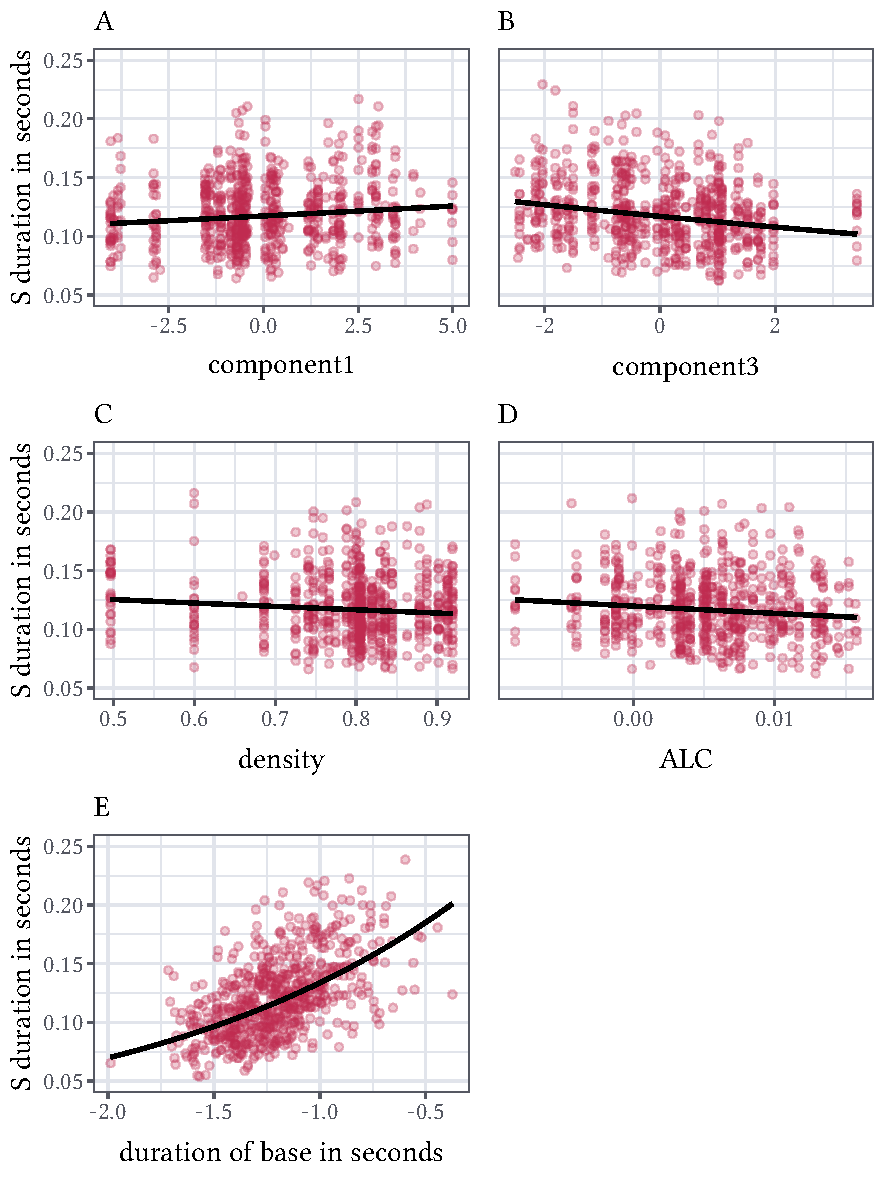
\includegraphics[]{figures/fig5.1.pdf}
    \caption{Partial effects of the numerical variables \textsc{Component1} (Panel A), \textsc{Component3} (Panel B), \textsc{density} (Panel C), \textsc{ALC} (Panel D), and \textsc{baseDurLog} (back-transformed, Panel E) included in model B, fitted to the log-transformed values of duration of /s/}
    \label{fig:5_1}
\end{figure}

The partial effects of the categorical variables included in the final model are illustrated in Figure \ref{fig:5_2} Pauses lead to longer /s/ durations (Panel A), which is most likely a case of phrase-final lengthening (e.g. \cite{Cooper1981}). There is also an effect of the following segment type, with /s/ being shorter when followed by a vowel (Panel B). This difference is significant for all consonant types being compared against vowels with the exception of fricatives. However, as there is only a small number of fricative cases in the data, this non-significant difference is potentially not meaningful. Lastly, there is an effect of preceding consonant on /s/ duration (Panel C). /s/ duration is significantly longer if preceded by a voiceless labiodental fricative /f/ or a voiceless velar stop /k/ as compared to cases where /s/ is preceded by a voiceless alveolar stop /t/. All other comparisons are non-significant.

\begin{figure}
    \centering
    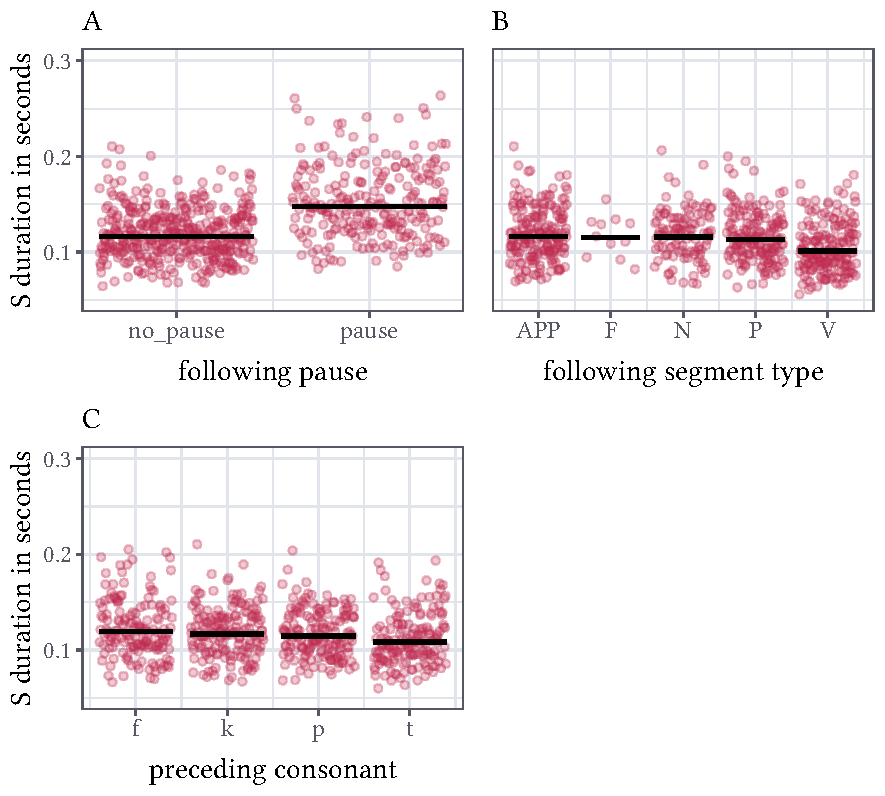
\includegraphics[]{figures/fig5.2.pdf}
    \caption{Partial effects of the categorical variables \textsc{pauseBin} (Panel A), \textsc{folType} (Panel B), and \textsc{preC} (Panel C) included in model B, fitted to the log-transformed values of duration of /s/}
    \label{fig:5_2}
\end{figure}

Let us turn to the variables of interest, i.e. those derived from the LDL network. \textsc{Component1} acts as a general measure of phonological certainty. High values of \textsc{Component1} come with high values of \textsc{path\_counts}, \textsc{path\_entropies}, and \textsc{ALDC}, indicating a high level of phonological uncertainty. At the other end of the \textsc{Component1} dimension, high values of \textsc{path\_sum} and \textsc{support} indicate a high level of phonological certainty. Higher uncertainty appears to lead to longer /s/ durations, while higher certainty appears to lead to shorter /s/ durations.

Recall from Section \ref{section05_2_5} that \textsc{Component3} relates to semantic activation diversity and to the presence of the plural suffix. Higher values of \textsc{Component3} indicate a higher level of semantic activation diversity. Higher levels of activation diversity then lead to shorter /s/ durations (see Panel B of Figure \ref{fig:5_1}). High values of \textsc{Component3} are positively correlated with the presence of plural /s/. It appears that the presence of plural makes words semantically more similar to each other as they share this meaning component. Hence, it is to be expected that plural words live in a space of greater semantic activation diversity. \textsc{Component3} is not only a measure of semantic activation diversity, but also indicates that plural pseudowords show a tendency of having a higher degree of semantic activation diversity as compared to monomorphemic pseudowords in general. \textsc{density} and \textsc{ALC} also tap into the semantics of pseudowords. That is, similar to \textsc{Component3}, higher values indicate higher levels of semantic activation diversity. These higher levels then lead to shorter /s/ durations.

\subsection{Model C: LDL measures only}\label{section05_3_3}

The final model of LDL measures only was fitted with effects of the following variables: \textsc{l1norm}, \textsc{ALC}, \textsc{NNC}, log-transformed base duration (\textsc{baseDurLog}), pause (\textsc{pauseBin}), following segmental type (\textsc{folType}), and preceding consonant (\textsc{preC}). The \textsc{speaker} variable was included as random intercept. The \textit{p}-values of the analysis of variance of the final model are given in Table \ref{tab:5.10}.

\begin{table}\fontsize{10}{11}
\caption{\textit{p}-values of fixed effects in model C, fitted to the log-transformed durations of /s/}
\label{tab:5.10}
\centering
\begin{tabular}{lrrrrrr} 
\lsptoprule
~          & Sum Sq & Mean Sq & NumDF & DenDF  & F.value & Pr(F)  \\ 
\midrule
\textsc{l1norm}     & 0.685  & 0.685   & 1     & 611.07 & 13.473  & 0.000  \\
\textsc{baseDurLog} & 6.047  & 6.047   & 1     & 627.51 & 118.901 & 0.000  \\
\textsc{pauseBin}   & 5.440  & 5.440   & 1     & 632.72 & 106.956 & 0.000  \\
\textsc{folType}    & 2.056  & 0.514   & 4     & 610.10 & 10.105  & 0.000  \\
\textsc{preC}       & 0.761  & 0.254   & 3     & 607.96 & 4.985   & 0.002  \\
\textsc{ALC}        & 0.534  & 0.534   & 1     & 615.51 & 10.504  & 0.001  \\
\textsc{NNC}        & 0.778  & 0.778   & 1     & 619.67 & 15.296  & 0.000  \\
\lspbottomrule
\end{tabular}
\end{table}

With a marginal R\textsuperscript{2} value of $0.41$, the fixed effects of this model explain 41 \% of variation within the data. The conditional R\textsuperscript{2} value of the model is $0.61$, that is the complete model accounts for 61 \% of variation.

The coefficients of the final model and their \textit{p}-values are given in Table \ref{tab:5.11}. The reference levels for the categorical covariates are: for \textsc{pauseBin} it is \texttt{no\_pause}; for \textsc{folType} it is \texttt{APP}, and for \textsc{preC} it is \texttt{f}.

\begin{table}\fontsize{10}{11}
\caption{Fixed-effect coefficients and \textit{p}-values as computed for model C (mixed-effects model fitted to the log-transformed duration of /s/)}
\label{tab:5.11}
\centering
\begin{tabular}{lrrrrr} 
\lsptoprule
~             & Estimate & SE    & df      & t-value & Pr(\textbar{}t\textbar{})  \\ 
\midrule
(Intercept)   & -2.334   & 0.320 & 625.440 & -7.301  & 0.000                      \\
\textsc{l1norm}        & -0.044   & 0.012 & 611.066 & -3.671  & 0.000                      \\
\textsc{baseDurLog}    & 0.624    & 0.057 & 627.514 & 10.904  & 0.000                      \\
\textsc{pauseBin}pause & 0.233    & 0.022 & 632.719 & 10.342  & 0.000                      \\
\textsc{foltype}\texttt{F}      & -0.019   & 0.073 & 613.088 & -0.267  & 0.790                      \\
\textsc{foltype}\texttt{N}      & -0.005   & 0.028 & 607.324 & -0.195  & 0.845                      \\
\textsc{foltype}\texttt{P}      & -0.023   & 0.024 & 607.817 & -0.950  & 0.343                      \\
\textsc{foltype}\texttt{V}      & -0.140   & 0.025 & 611.952 & -5.693  & 0.000                      \\
\textsc{preC}\texttt{k}         & -0.029   & 0.027 & 607.726 & -1.058  & 0.291                      \\
\textsc{preC}\texttt{p}         & -0.053   & 0.027 & 607.478 & -1.950  & 0.052                      \\
\textsc{preC}\texttt{t}         & -0.101   & 0.028 & 608.068 & -3.632  & 0.000                      \\
\textsc{ALC}           & -6.663   & 2.056 & 615.511 & -3.241  & 0.001                      \\
\textsc{NNC}           & 1.221    & 0.312 & 619.671 & 3.911   & 0.000                      \\
\lspbottomrule
\end{tabular}
\end{table}

As for both other final models, the predictor strength of the individual predictors was checked. This procedure resulted in the hierarchy of predictor strength given in \ref{ex:5.3}. That is, the decrease in R\textsuperscript{2} is greatest when removing \textsc{baseDurLog}, followed by \textsc{pauseBin}, and so forth. 

\ex.
\label{ex:5.3}
\textsc{baseDurLog >> pauseBin >> folType >> NNC >> l1norm >> ALC >> preC}

Figure \ref{fig:5_3} displays the effect on /s/ duration of the numerical variables included in the model. Base duration shows an identical effect as compared to model B in Section \ref{section05_3_2}, i.e. longer base durations come with longer /s/ durations. 

\begin{figure}
    \centering
    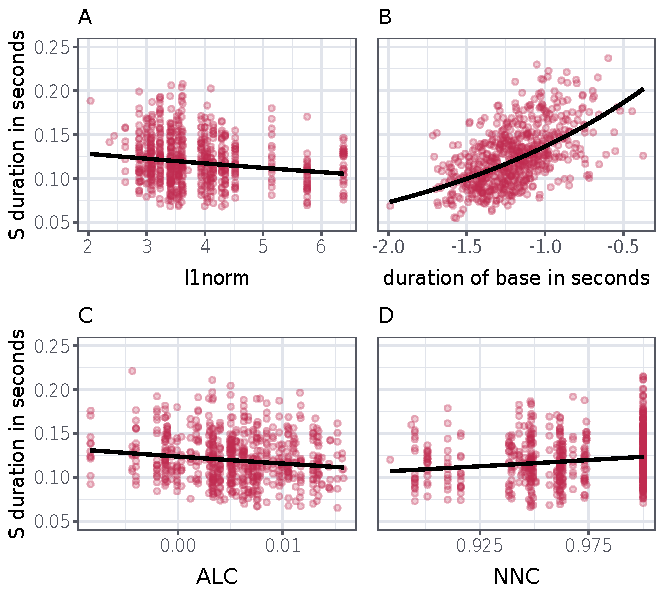
\includegraphics[]{figures/fig5.3.pdf}
    \caption{Partial effects of the numerical variables \textsc{l1norm} (Panel A), \textsc{baseDurLog} (back-transformed, Panel B), \textsc{ALC} (Panel C), and \textsc{NNC} (Panel D) included in model C, fitted to the log-transformed values of duration of /s/}
    \label{fig:5_3}
\end{figure}

Figure \ref{fig:5_4} shows the effect on /s/ duration of the categorical variables included in the model. Pauses again come with longer /s/ durations, and /s/ is shorter if followed by a vowel. There is also an effect of the preceding consonant, with /s/ duration being significantly longer if preceded by a voiceless labiodental fricative /f/ or a voiceless velar stop /k/ as compared to cases where /s/ is preceded by a voiceless alveolar stop /t/. These results are generally in line with those by the analysis in the previous section.

\begin{figure}
    \centering
    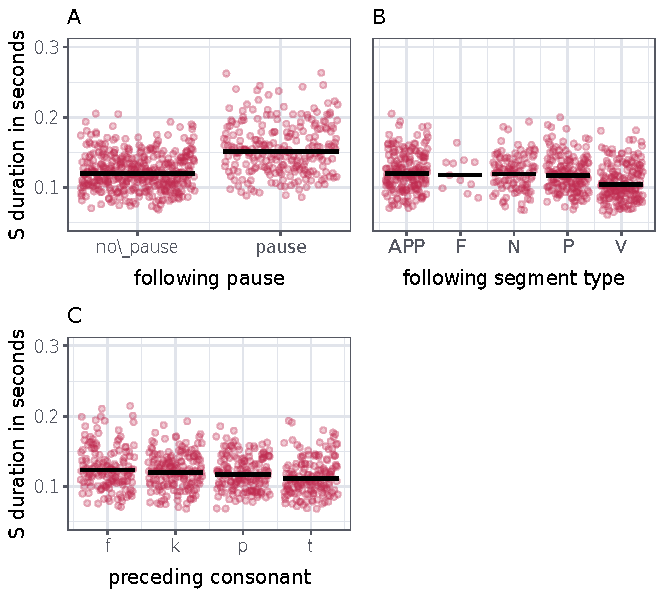
\includegraphics[]{figures/fig5.4.pdf}
    \caption{Partial effects of the categorical variables \textsc{pauseBin} (Panel A), \textsc{folType} (Panel B), and \textsc{preC} (Panel C) included in model C, fitted to the log-transformed values of duration of /s/}
    \label{fig:5_4}
\end{figure}

Taking a closer look at the variables of interest, one finds that higher values of \textsc{l1norm} and \textsc{ALC}, i.e. higher semantic activation diversity, lead to shorter /s/ durations. As in model B, higher levels of semantic activation diversity come with shorter /s/ durations. For \textsc{NNC}, it is found that /s/ duration is longer if a pseudoword is semantically similar to a real word.

\section{Discussion}\label{section05_4}

The production study presented in Chapter \ref{chapter04} of this book as well as previous studies (\cite{Zimmermann2016, Plag2017, Seyfarth2017, Tomaschek2019, Plag2020}) reported that there are significant differences in the acoustic duration between different types of word-final /s/ in English. Such durational differences challenge established feed-forward theories of morphology-phonology interaction (e.g. \cite{Chomsky1968, Kiparsky1982}) as well as theories of psycholinguistics (e.g. \cite{Levelt1999, Roelofs2019, Turk2020}). The present study investigated whether measures derived on the basis of a discriminative learning theory are predictive of /s/ durations in pseudowords. In particular, LDL networks that model the production of a word based on its relation to the rest of the lexicon were implemented.

The predictive possibilities of LDL measures were explored by fitting three different models: a) a model based on the traditional predictors as used in previous studies (\cite{Plag2017,,Tomaschek2019}) and most importantly in the production study reported in this book; b) a model with LDL measures and a variable \textsc{typeOfS} specifying the presence or absence of an affix; and c) a model with LDL measures but without a variable specifying the presence or absence of an affix. Both models with LDL measures show that such measures are predictive of /s/ durations. This result is the most important of the present study. While traditional variables such as lexical frequencies, bigram frequencies, transitional probabilities, or neighbourhood densities measure important lexical properties, it is unclear why they would manifest themselves in a particular morphological effect in speech production. In LDL such effects can emerge through the mapping of form and meaning in a clearly defined process of discriminative learning.

All regression models showed a similar hierarchy of predictor strength for the variables included in the models. For the traditional model A, \textsc{typeOfS} is the third-strongest predictor of /s/ duration and for model B this spot is taken by \textsc{Component3}, while there is no comparable variable included in model C. Comparing the variance explained by the fixed effects of the different models, one finds that the traditional model accounts for most variation, i.e. 43 \%, while the LDL model including the \textsc{typeOfS} variable accounts for 42 \%, and the LDL model without the \textsc{typeOfS} variable accounts for 41 \% of variation. Thus, in terms of marginal R\textsuperscript{2} values, all three models are close to each other. To check whether these differences in marginal R\textsuperscript{2} values are of significance, the three models were refitted to the untrimmed data set and then compared with a likelihood-ratio test. The results suggest that there is no significant difference between the traditional model and the LDL model including the \textsc{typeOfS} variable. However, the LDL model without the \textsc{typeOfS} variable shows a significantly worse fit ($p<0.01$). This seems to indicate that the LDL measures do not capture the full amount of the variance that is captured by the variable \textsc{typeOfS}. This means that there is still something about the morphological function that translates into duration and that is not properly modelled by the associative measurements of the learning network. The same problem holds, incidentally, for the traditional model (model A), in which the usual lexical measures (such as lexical frequencies, neighbourhood densities, etc.) and phonetic covariates (such as pauses, speech rate, etc.) are also not able to cover all durational variance. The morphological residue in both types of analysis remains a conundrum that calls for more sophisticated approaches in future research.

The LDL measures included in the final models are either concerned with semantic activation diversity (\textsc{Component3}, \textsc{ALC}, \& \textsc{density} in model B; \textsc{l1norm} \& \textsc{ALC} in model C), semantic similarity (\textsc{NNC} in model C) or with phonological certainty (\textsc{Component1} in model B).

Higher degrees of semantic activation diversity come with shorter /s/ durations. This effect is similar to the one which was reported by \citet{Tucker2019Sims} in a study on stem vowels and \citet{Tomaschek2019} in their NDL study on /s/ duration. A higher degree of activation diversity makes it ``more difficult to discriminate the targeted outcome from its competitors" (\cite[27]{Tomaschek2019}). As for production, a prolongation of the acoustic signal is dysfunctional if the prolongation maintains or increases the discrimination problem instead of contributing to resolving it (\cite{Tomaschek2019}).

In the model without \textsc{typeOfS} as predictor variable, \textsc{NNC} (i.e. a pseudoword’s semantic similarity to its closest semantic real word neighbour) emerges as significant (see model C). Why so? As reported in Section \ref{section05_2_5}, the \textsc{typeOfS} variable and \textsc{NNC} are strongly negatively correlated ($rho = -0.89$). Post-hoc analysis shows that plural /s/ has significantly lower \textsc{NNC} values as compared to non-morphemic /s/ (Wilcoxon test,  $p<0.001$). It therefore appears that \textsc{NNC} takes over the role of differentiating between plural and non-morphemic /s/ in model C.

As for phonological certainty, one finds that higher phonological certainty comes with shorter /s/ durations, while higher phonological uncertainty comes with longer /s/ durations. Shorter durations in contexts of high phonological certainty may be related to effects of frequency, i.e. highly frequent forms are produced with higher certainty and are thus shorter. 

The results of the present study may bring up further questions. First, are the predictive measures found for word-final /s/ duration in pseudowords also predictive for word-final /s/ duration in real words? The NDL implementation of \citet{Tomaschek2019} suggests that they are, but LDL networks still need to be implemented. It would be especially interesting to model those data sets that have yielded seemingly contradictory effects. Second, taking into account that the specification of \textsc{typeOfS} in the modelling process leads to a significantly better model fit, one may ask what the underlying reasons for this significant effect are. This then automatically leads to another question: Is it possible to catch the effect of the \textsc{typeOfS} specification in terms of (new) LDL measures? 

To summarise, this study was the first to investigate durational differences between different types of word-final /s/ (non-morphemic versus plural /s/) in pseudowords by means of an LDL implementation, measures, and resulting statistical analyses. The findings yielded important evidence on the question of how such durational differences come to be, i.e. they can be predicted based on their pseudoword’s relations to the lexicon. It was demonstrated that durational differences emerge from the pseudoword’s resonance with the lexicon by way of differing degrees of semantic activation diversity and phonological uncertainty. These manifestations of the relations to other words in the lexicon in turn are the result of discriminative learning.
